\section{State-of-the-Art in Verification of Concurrent Software}\label{sec:sota}

\begin{figure}[b]
\fcolorbox{\leadingcolor}{White}{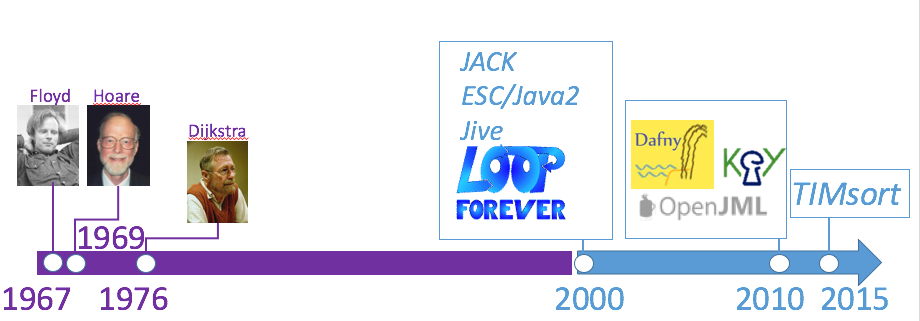
\includegraphics[width=\textwidth]{timeline_sequential.png}}
\caption{Development of Sequential Software Verification}\label{fig:sequential}
\end{figure}

\subsection{Software Correctness}
\addcontentsline{toc}{subsubsection}{Software Correctness}

The quest for software correctness is an old tale (see Figure~\ref{fig:sequential} for a historic overview). Already in the sixties, in the early days of computing, Floyd and Hoare realised that it is actually possible to prove that a program behaves as intended~\cite{Hoare69,Floyd67}. Given a small code fragment, and a specification of what the fragment is supposed to do, a collection of simple proof rules was devised, which can be used to establish whether a program behaves as specified. By applying the proof rules, auxiliary proof obligations in first-order logic are generated. If the proof obligations can be proven, we can conclude that the program satisfies its specification. This approach, called Floyd-Hoare  or Hoare logic, still forms the basis for many techniques to reason about program behaviour (usually implemented using Dijkstra's predicate transformer semantics~\cite{Dijkstra76}).

For a long time, program verification remained a pen-and-paper activity. However, around the year 2000, several groups started working on the development of tools to support this kind of verification~\cite{Huisman01,BergJ01,BartheBCGHLPR07,BeckertHS07,CokK04,MeyerP00}. There are several technical reasons behind the coordination of these developments:
\begin{itemize}[topsep=0pt,noitemsep]
\item the emergence of Java meant that there was a popular and widely-used programming language with a reasonably well-defined semantics, amenable to formal reasoning;
\item in addition, computing power had increased, which made it actually feasible to build efficient tools to reason about non-trivial programs; and
\item there was tremendous progress in automated verification technology for first-order logic, which enabled automatic discharge of auxiliary proof obligations, culminating in modern, very powerful SMT solvers.
\end{itemize}
Since then, work on these program verification tools has progressed, resulting in tools such as OpenJML~\cite{Cok14}, CodeContracts~\cite{Logozzo11,FahndrichLLB12}, and the most recent versions of KeY~\cite{Ahrendt16}, which are now being used in teaching, integrated in standard development environments, and to verify or find bugs in non-trivial algorithms, such as TIMsort~\cite{DeGouwRBBH15}. 

Despite the enormous progress that has been made, there are still many open challenges in this area~\cite{HaehnleH18}. One important open challenge for program verification is that it still requires a substantial level of expertise, in particular because of the high number of auxiliary annotations that have to be provided to guide the proving process (see for example the solutions to the VerifyThis program verification challenges at \url{http://www.verifythis.org}). 


\subsection{Verification of Concurrent Software}
\addcontentsline{toc}{subsubsection}{Verification of Concurrent Software}
 All techniques mentioned above focus on proving local safety properties of sequential programs, \emph{i.e.}, with a single thread of execution, but cannot specify or effectively prove properties on the global program behaviour of concurrent or distributed software.  Thus, extending program verification techniques to enable reasoning about programs with multiple threads of execution is a necessary step to ensure the reliability of realistic programs, see Figure~\ref{fig:concurrent} for a historic overview.

\begin{figure}[t]
\fcolorbox{\leadingcolor}{White}{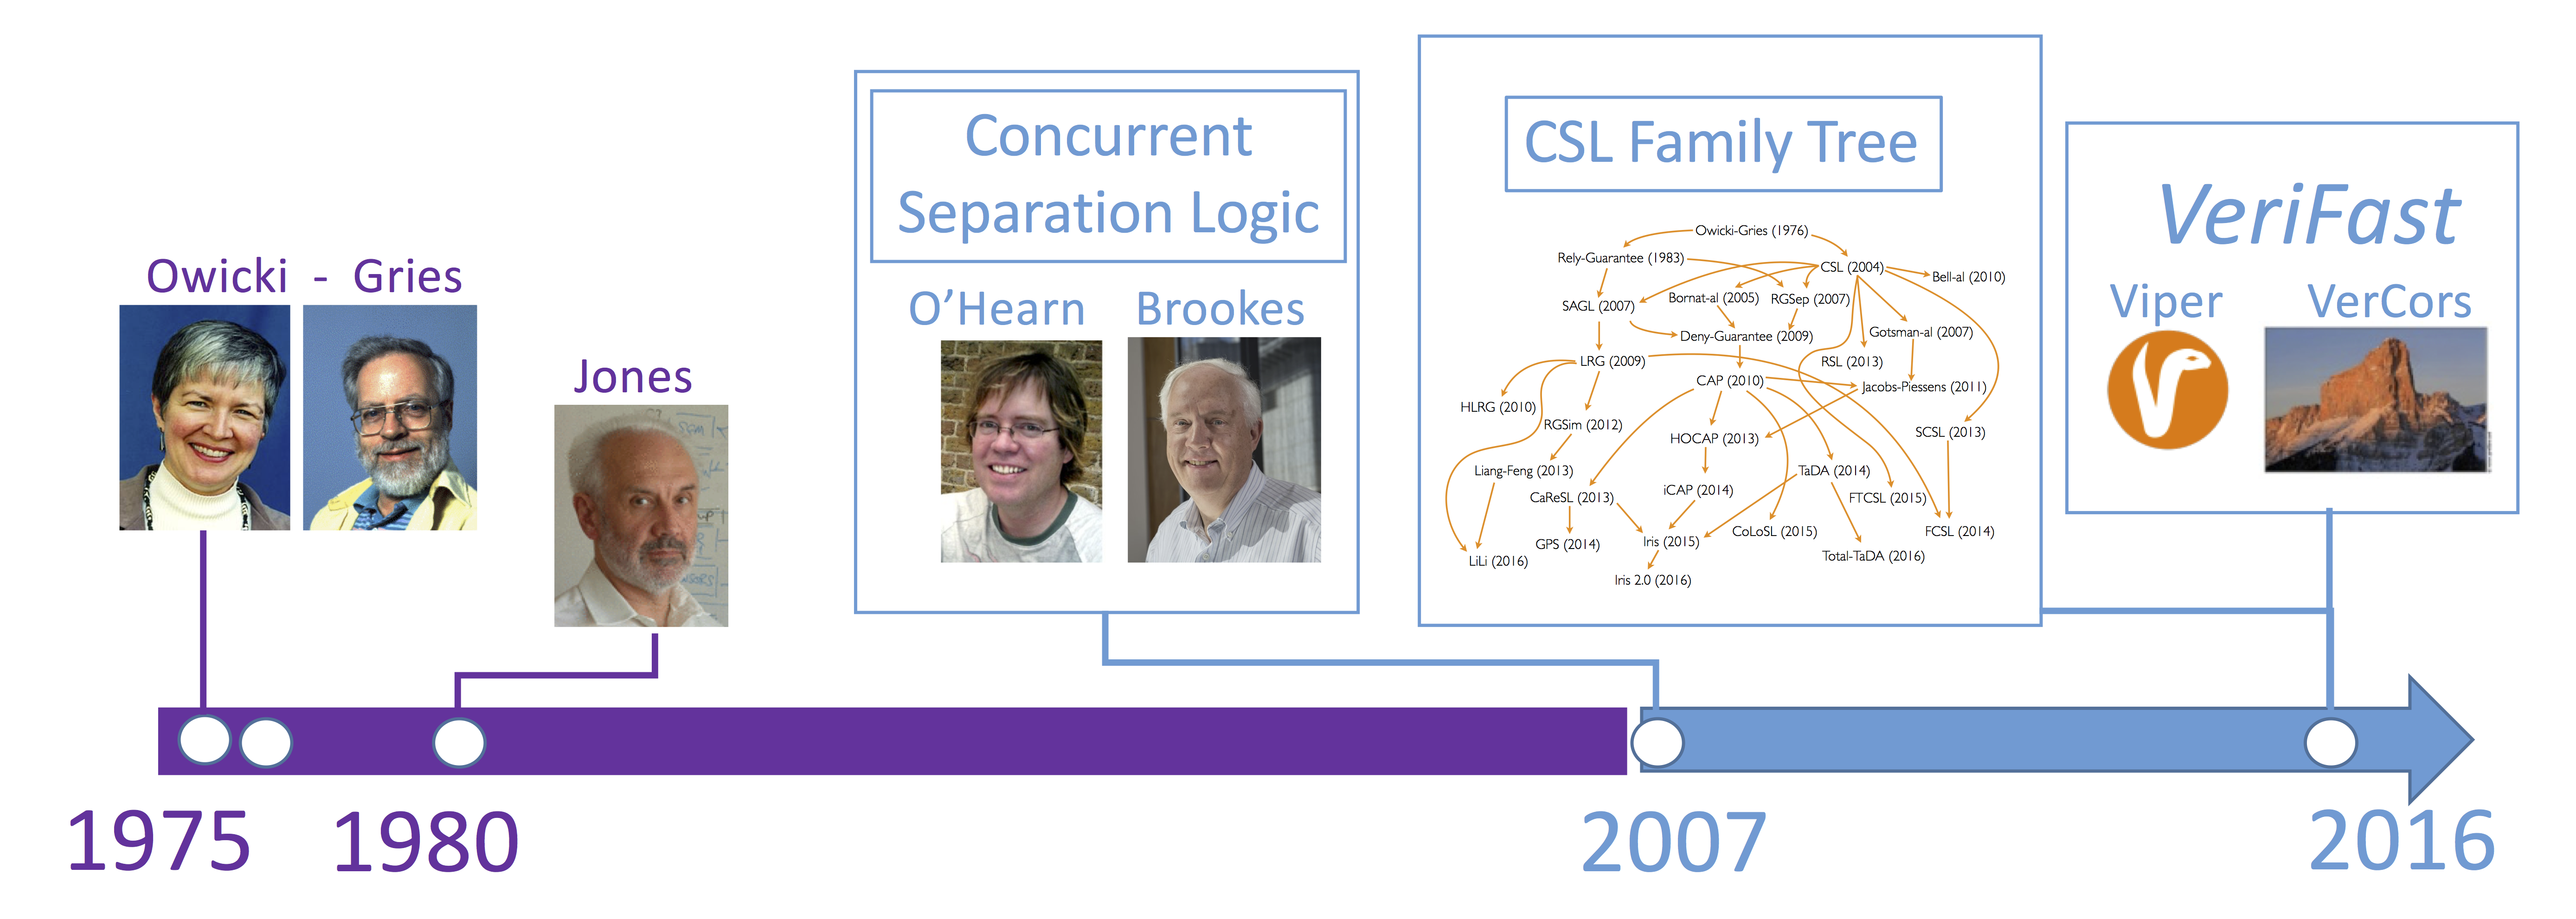
\includegraphics[width=\textwidth]{timeline_concurrent.png}}
\caption{Development of Concurrent Software Verification}\label{fig:concurrent}
\end{figure}

Already in the 70s, Owicki and Gries proposed a technique to extend program logic to reason about concurrent programs~\cite{OwickiG75}. Their technique required annotations for each atomic step in the program, and a proof that these annotations could not be invalidated by any atomic step made by other program threads, thus resulting in a non-modular verification technique with an exponential number of proof obligations.  In particular, if a verified program is extended with a new thread, also the existing threads have to be reverified. In 1980, Jones proposed a modular verification technique for concurrent programs, called rely-guarantee reasoning~\cite{Jones83}. In rely-guarantee reasoning the verifier explicitly specifies the steps that are allowed for the environment, which requires thorough understanding of the application at hand.

About 10 years ago, Concurrent Separation Logic (CSL) was invented~\cite{OHearn07,Brookes07} (Brookes and O'Hearn received the G\"odel prize 2016 for this achievement).  This was an important step for the verification of concurrent software, as it enabled thread-modular verification. Originally, separation logic was proposed as an extension of classical Hoare logic to reason about pointer programs, by explicitly considering which memory locations are relevant for what part of the program~\cite{OHearnRY01,OHearnYR04}. This characteristic makes it also extremely suitable to reason about concurrent programs: if we can prove that two threads work on disjoint parts of the memory, then we know that they cannot interfere with each other. 

The invention of concurrent separation logic led to a whole plethora of techniques and logics to reason about concurrent software, focusing on different aspects, see~\cite{BrookesO16} for an overview. 

In one line of work, more and more advanced logics are proposed, grouped in the CSL family tree~\cite{BrookesO16}. This contains for example a combination of rely guarantee and separation logic~\cite{VafeiadisP07}, (impredicative) concurrent abstract predicates~\cite{Dinsdale-YoungDGPV10,SvendsenB14}, TaDa (a logic for time and data abstraction)~\cite{daRochaPintoDG14,daRochaPintoDG15},  fine-grained concurrent separation logic~\cite{NanevskiLSD14,SergeyNB15}, a combination of monoids and invariants~\cite{JungSSSTBD15,KrebbersJBJDB17}, and reasoning based on linearisation points~\cite{Vafeiadis10,HemedRV15}, with the aim of finding a generic logic, which can be used to verify the behaviour of all concurrent programs. So far, these approaches are still fairly theoretic, and require a high level of expertise. Some of these logics are formalised in Coq, with suitable tactics to use them inside Coq.  Further, they 
are usually developed for relatively simple core programming languages, and focus on small but intricate examples. 

In another line of work, the focus is on developing practical techniques to reason about commonly used programs, using various synchronisation methods, support for dynamic thread creation, reentrant locks etc. This has been the focus of our work on the VerCors tool set~\cite{AmighiHHH15,AmighiBHZ12,AmighiBDHMZ14,BlomDHO17IFM}, where we developed techniques (with tool support) to reason about multi-threaded Java and OpenCL programs. This is also the aim of the VeriFast tool, for verification of single- and multithreaded C and Java programs~\cite{JacobsP08,SmansJP13} and the Viper framework, which provides support for separation logic-based reasoning for a low-level intermediate language~\cite{JKMNSS14,MuellerSS16}. In particular, our VerCors tool is build on top of the Viper framework. Some of the more theoretical results on verification of concurrent software are (partially) integrated in these techniques. 

By now, there is a plethora of logics to verify specific core properties about concurrent software, such as that the program is free of data races. The next challenge is to efficiently prove properties about the \emph{global functional behaviour} of a realistic concurrent program. 






% \subsection{Verification of Distributed Software}
% \addcontentsline{toc}{subsubsection}{Verification of Distributed Software}

% In the literature, verification of distributed software has followed a different approach. Most work has focused on the verification of distribution aspects at a highly abstract level, where the programs are modelled as abstract processes, \emph{e.g.}, using process algebras~\cite{Hoare78,Milner80,BergstraPS01} or \(\pi\)-calculus~\cite{Milner99,SangiorgiW01}, and the gap with concrete program code is huge. There also exist some proposals to use separation logic to reason about a language with process algebraic communication operators~\cite{HoareO08,BellAW10}, but these are for very basic core programming languages.

% \begin{highlightbox}
% It is an open challenge to bridge the gap between the verification of models of distributed program and verification of actual distributed program code.
% \end{highlightbox}

% In the context of my TOP project VerDi, we have sketched how histories and futures also have the potential to reason about distributed programs~\cite{OortwijnBH16}. The communication actions between the different processes are abstracted into actions, and for each process a history or future is used to describe the control flow of the process. This transforms the software verification problem into a verification problem of communicating processes at the process algebra level. However, to make this approach practical, we still need suitable compositional verification technique at the abstract level, as will be developed within Mercedes.


\subsection{Concurrent Software in Industrial Practice}
Because of high demands on software performance, industry is using concurrency more and more in their daily practice. However, for many companies, reliability of the software they develop is very important: if their software is misbehaving, they risk losing the confidence of their customers. Therefore, we see that companies are often quite conservative in their use of concurrency: they use well-known programming patterns, reuse existing libraries as much as possible, and try to isolate the concurrency-related aspects to a small part of their application.

Software developers need effective verification techniques to improve the quality and reliability of their concurrent software.
We believe that to develop these techniques, the ultimate challenge is not in finding a logic that can reason about all possible concurrent programs.
Instead, the challenge is to develop techniques that can be used efficiently on many common concurrent programming patterns, and that can be used to detect bugs quickly and effectively, without requiring too many user interventions, and without too many false positives. This conviction is what drives our research: we aim at developing techniques that can help software developers in their daily software development practice to improve the quality of the software they are producing.

